\documentclass[aspectratio=169]{beamer}
\usepackage[utf8]{inputenc} % codificacao de caracteres
\usepackage[T1]{fontenc}    % codificacao de fontes
\usepackage[english]{babel}  % idioma
\usepackage{graphics,amssymb,amsfonts,amsmath,xfrac}
\usepackage{tikz}
\usepackage{enumerate,hyperref}
\usepackage{palatino}	% Fonte sem serifa
\usepackage{ragged2e}	% Paragrafo justificado
%\usepackage{minted}	% Highlight para codigos de programacao
\usepackage{booktabs} % tabelas
\usepackage{multicol}
\usepackage{multirow}
%\usepackage[table]{xcolor}


% Veja mais temas e cores em http://www.hartwork.org/beamer-theme-matrix/
\usetheme{Montpellier}         % tema
\usecolortheme{orchid}      % cores
\usefonttheme[onlymath]{serif} % fonte modo matematico
% Colocando numero de paginas no slide
\setbeamertemplate{footline}[frame number]



\DeclareGraphicsExtensions{.pdf,.jpg,.png} % compilamos apenas com pdflatex
\graphicspath{{figuras/}} % caminho onde as figuras estarao disponiveis




% ---------------------------------------------------------------------------- %
% T�tulo                                                                       %
% ---------------------------------------------------------------------------- %

\title[\sc{Teoria de Circuitos Eletrônicos 1}]{\LARGE Aula 7 - Exercise Class 2}
\author[Prof. Marcelino Andrade]{Prof. Marcelino Andrade}
\institute{Faculdade UnB Gama} % opcional
\date{\today}

\begin{document}
\justifying % Paragrafo justificado
\pagebreak

\begin{frame}
  \titlepage
\end{frame}


% ----------------- NOVO SLIDE --------------------------------
\begin{frame}{Contents\newline}

\tableofcontents
\begin{center}	
     		Fundamentals of Electric Circuits (Alexander and Sadiku), 4th Edition			
\end{center}	
\end{frame}

% ----------------- NOVA SECÇÂO -----------------------------
\section{Section 4.3 Superposition}
% ----------------- NOVO SLIDE --------------------------------
\begin{frame}[fragile]
	\frametitle{Superposition}
\begin{tabular}{ll}
	\begin{columns}
		\begin{column}{1\textwidth}  %%<--- here
		\textbf{Problem 4.19} - Use superposition to solve for $v_{x}$ in the circuit of Figure below.\\
		\begin{center}
    			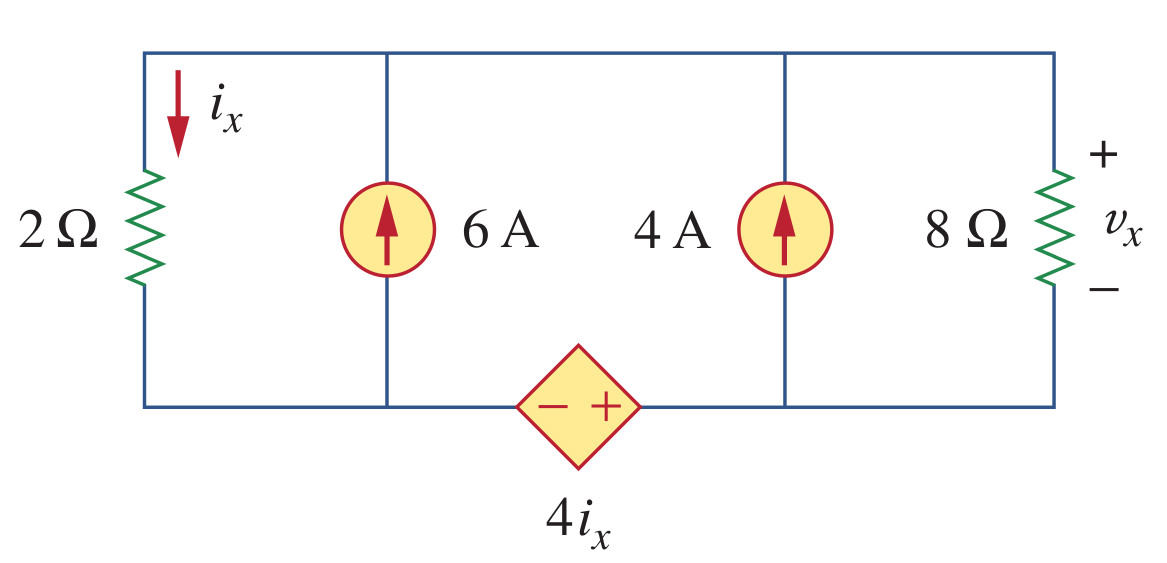
\includegraphics[height=3.6cm]{figure4.png}	
		\end{center}	
		\scalebox{0.8}{Answer: $v_{x}= -26.67V$.}
		\end{column}
	\end{columns}
\end{tabular}
\end{frame}

% ----------------- NOVA SECÇÂO -----------------------------
\section{Section 4.4 Source Transformation}
% ----------------- NOVO SLIDE --------------------------------
\begin{frame}[fragile]
	\frametitle{Source Transformation}
\begin{tabular}{ll}
	\begin{columns}
		\begin{column}{1\textwidth}  %%<--- here
		\textbf{Problem 4.31} - Determine $v_{x}$ in the circuit of Figure below using source transformation.\\
		\begin{center}
    			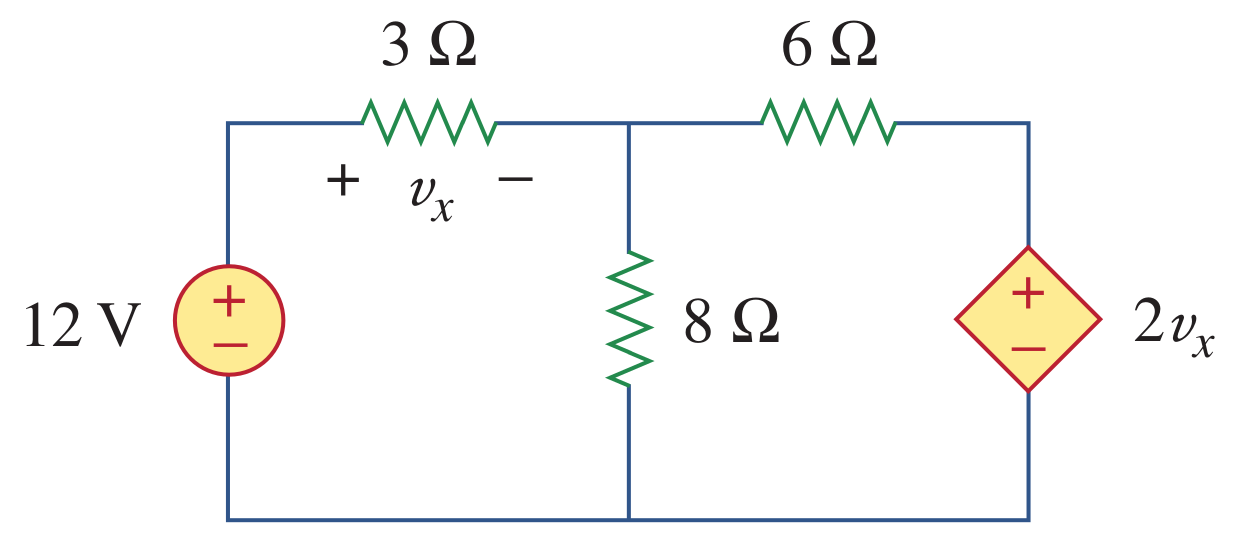
\includegraphics[height=3.6cm]{figure5.png}	
		\end{center}	
		\scalebox{0.8}{Answer: $v_{x}= 3.652V$.}
		\end{column}
	\end{columns}
\end{tabular}
\end{frame}

% ----------------- NOVA SECÇÂO -----------------------------
\section{Section 4.5 and 4.6 Thevenin’s and Norton's Theorems}
% ----------------- NOVO SLIDE --------------------------------
\begin{frame}[fragile]
	\frametitle{Thevenin’s Theorem}
\begin{tabular}{ll}
	\begin{columns}
		\begin{column}{1\textwidth}  %%<--- here
		\textbf{Problem 4.39} - Obtain the Thevenin equivalent at terminals $a-b$  of the circuit in Figure below.\\
		\begin{center}
    			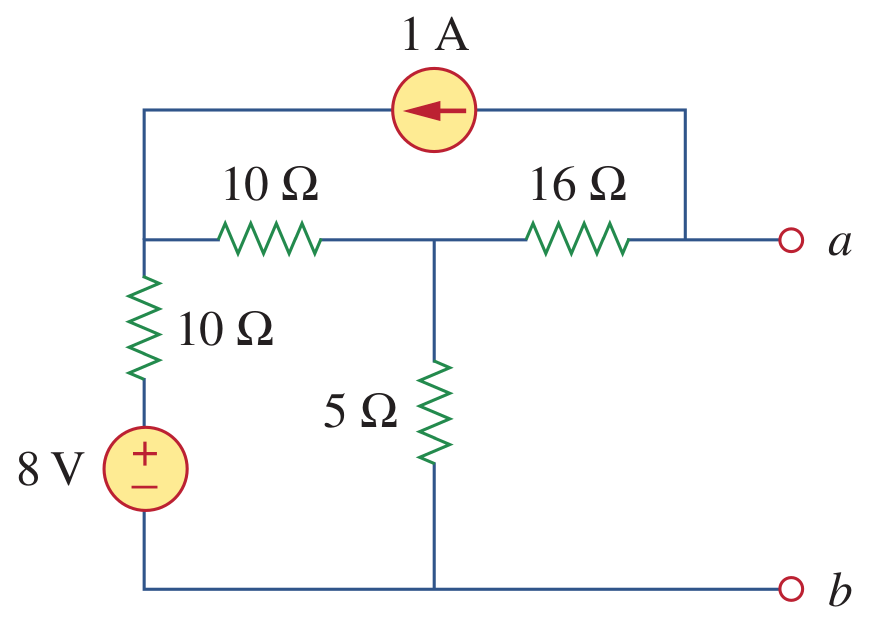
\includegraphics[height=3.6cm]{figure6.png}	
		\end{center}	
		\scalebox{0.8}{Answer: $v_{t}= -16.4V \ and \ R_{t}=20\Omega$}
		\end{column}
	\end{columns}
\end{tabular}
\end{frame}

% ----------------- NOVO SLIDE --------------------------------
\begin{frame}[fragile]
	\frametitle{Norton’s Theorem}
\begin{tabular}{ll}
	\begin{columns}
		\begin{column}{1\textwidth}  %%<--- here
		\textbf{Problem 4.55} - Obtain the Norton equivalent at terminals $a-b$ of the circuit in Figure below.\\
		\begin{center}
    			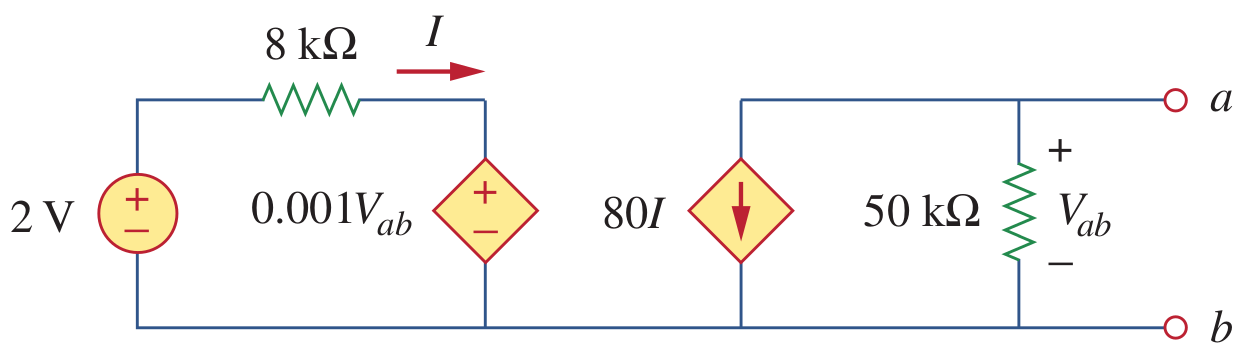
\includegraphics[height=3.6cm]{figure7.png}	
		\end{center}	
		\scalebox{0.8}{Answer: $i_{n}= -20mA \ and \ R_{n}=100K\Omega$}
		\end{column}
	\end{columns}
\end{tabular}
\end{frame}


% ----------------- NOVA SECÇÂO -----------------------------
\section{Section 4.8 Maximum Power Transfer}
% ----------------- NOVO SLIDE --------------------------------
\begin{frame}[fragile]
	\frametitle{Maximum Power Transfer}
\begin{tabular}{ll}
	\begin{columns}
		\begin{column}{1\textwidth}  %%<--- here
		\textbf{Problem 4.71} - For the circuit in Figure below, what resistor connected across terminals $a-b$ will absorb maximum power
from the circuit? What is that power?\\
		\begin{center}
    			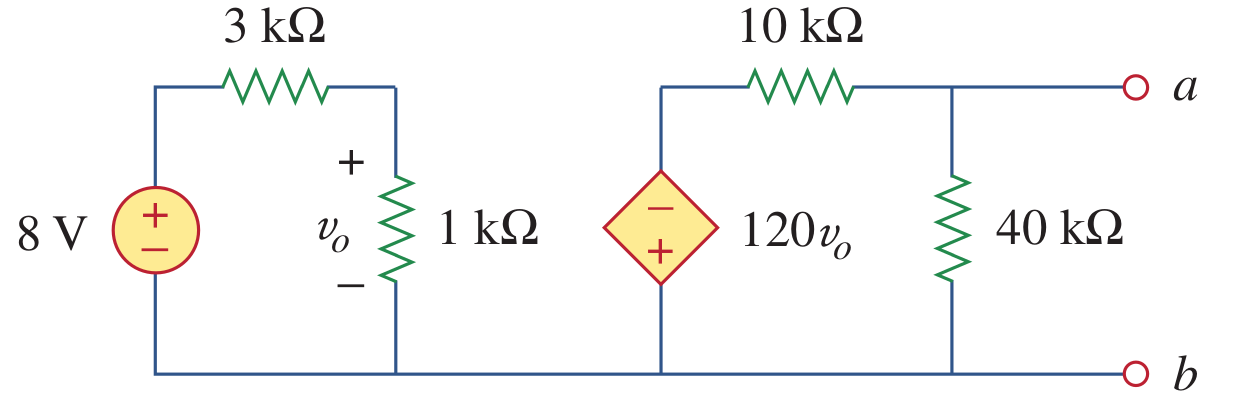
\includegraphics[height=3.6cm]{figure8.png}	
		\end{center}	
		\scalebox{0.8}{Answer: $R_{L}= 8K\Omega \ and \ P_{L}=1.152W$}
		\end{column}
	\end{columns}
\end{tabular}
\end{frame}
%----------------- NOVA SECÇÂO -----------------------------
\section{Section 5.2 Operational Amplifiers}
% ----------------- NOVO SLIDE --------------------------------
\begin{frame}[fragile]
	\frametitle{Operational Amplifiers}
\begin{tabular}{ll}

\begin{columns}
  \begin{column}{1\textwidth}
\textbf{Problem 5.7} - The op amp in Figure below has $R_{i}=100K\Omega$,
$R_{o}=100\Omega$, $A=100,000$. Find the differential voltage $v_{d}$ and the output voltage $v_{o}$.\\
  \end{column}
\end{columns}\\

	\begin{columns}
		\begin{column}{.4\textwidth}  %%<--- here
		\begin{center}
    			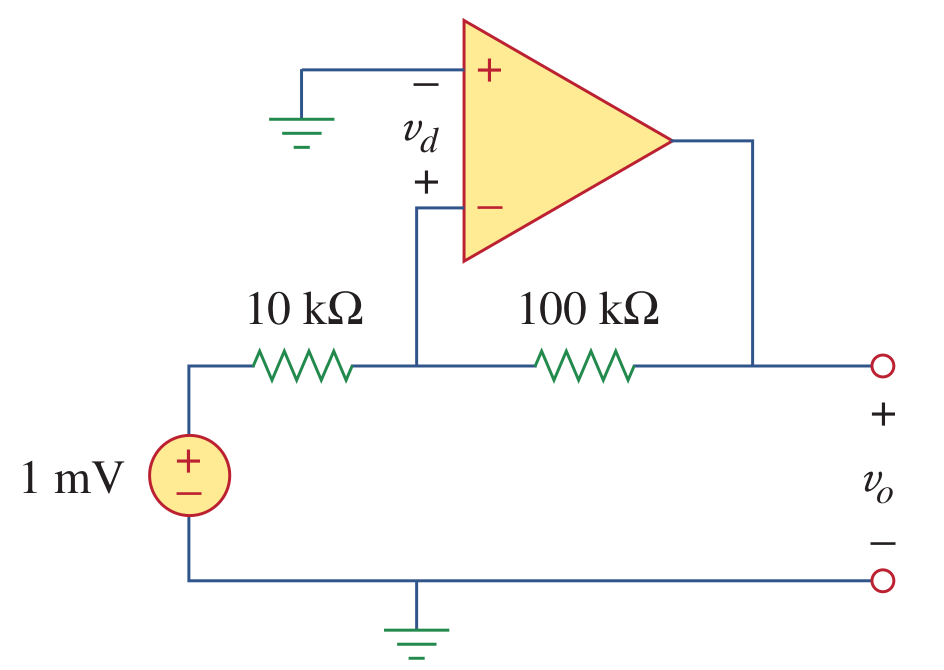
\includegraphics[height=3.6cm]{figure9.png}
		\end{center}	
		\scalebox{0.8}{Answer: $v_{d}= -100nV \ and \ v_{o}=-10mV$}
		\end{column}
		\begin{column}{.5\textwidth}  %%<--- here
		\begin{center}
   			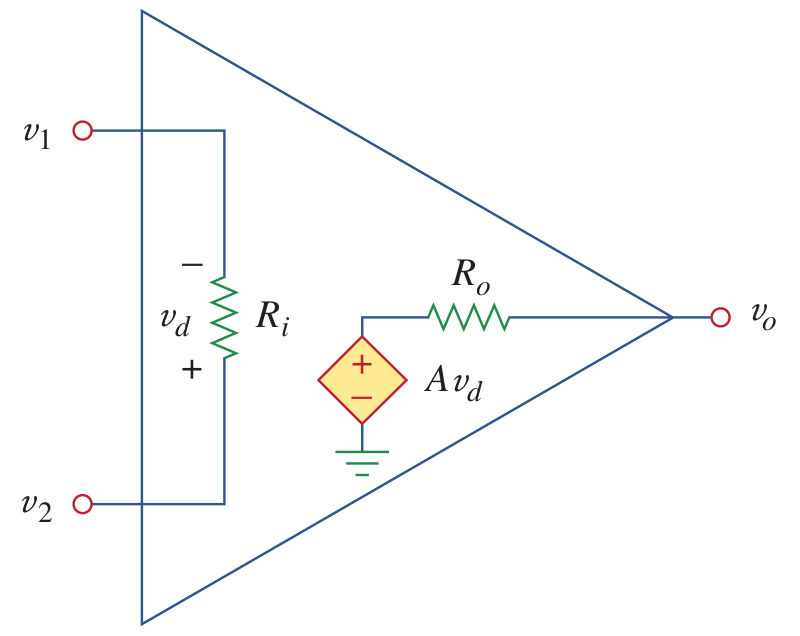
\includegraphics[height=2.6cm]{figura06m.png}	

		\end{center}	
		
		\end{column}

		
		
		
		
	\end{columns}
\end{tabular}
\end{frame}
% ----------------- NOVA SECÇÂO -----------------------------
\section{Section 5.3 Ideal Op Amp}
% ----------------- NOVO SLIDE --------------------------------
\begin{frame}[fragile]
	\frametitle{Ideal Op Amp}
\begin{tabular}{ll}
	\begin{columns}
		\begin{column}{1\textwidth}  %%<--- here
		\textbf{Problem 5.13} - Find $v_{o}$ and $i_{o}$ in the circuit of Figure below.\\
		\begin{center}
    			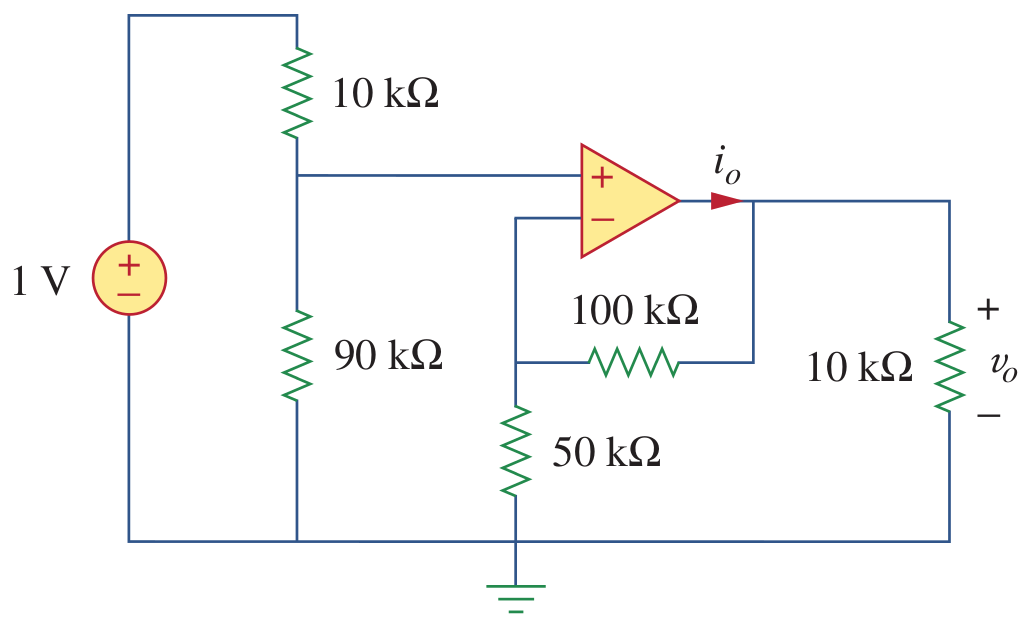
\includegraphics[height=3.6cm]{figure11.png}	
		\end{center}	
		\scalebox{0.8}{Answer: $v_{o}= 2.7V \ and \ i_{0}=288\mu V$}
		\end{column}
	\end{columns}
\end{tabular}
\end{frame}
% ----------------- NOVO SLIDE --------------------------------
\begin{frame}[fragile]
	\frametitle{Ideal Op Amp}
\begin{tabular}{ll}
	\begin{columns}
		\begin{column}{1\textwidth}  %%<--- here
		\textbf{Problem 5.17} - Calculate the gain \scalebox{1.2}{$\sfrac{v_{o}} {v_{i}}$} when the switch in Figure below is in: (a) position 1, (b) position 2 and (c) position 3.\\
		\begin{center}
    			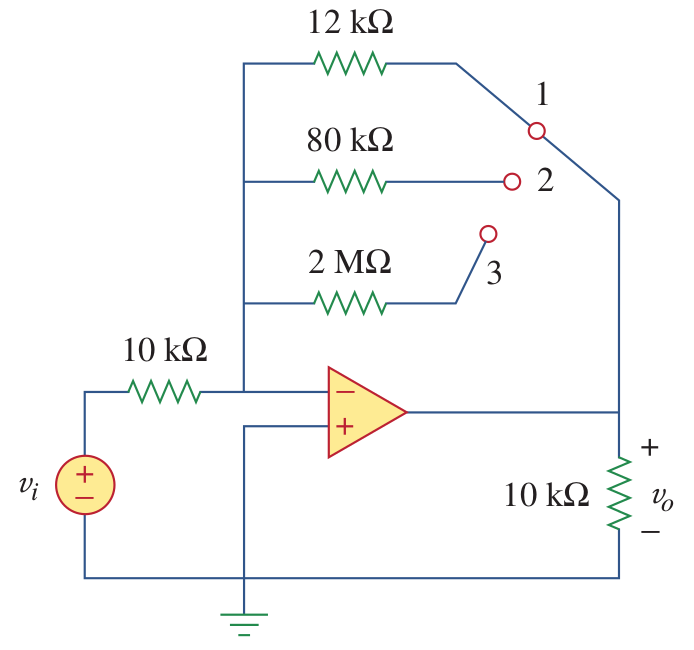
\includegraphics[height=3.6cm]{figure10.png}	
		\end{center}	
		\scalebox{0.8}{Answer: $(a)\ \frac{v_{o}} {v_{i}}=-1.2, (b)\ \frac{v_{o}} {v_{i}}=-8,\ and \ (a)\ \frac{v_{o}} {v_{i}}=-200$}
		\end{column}
	\end{columns}
\end{tabular}
\end{frame}

% ----------------- NOVA SECÇÂO -----------------------------
\section{Section 5.4 Inverting, Noninverting, Summing and Difference Amplifiers}
% ----------------- NOVO SLIDE --------------------------------
\begin{frame}[fragile]
	\frametitle{Inverting, Noninverting, Summing and Difference Amplifiers}
\begin{tabular}{ll}
	\begin{columns}
		\begin{column}{1\textwidth}  %%<--- here
		\textbf{Problem 5.33} - Refer to the op amp circuit in Figure below. Calculate $i_{x}$ and the power dissipated by the $3K\Omega$ resistor.\\
		\begin{center}
    			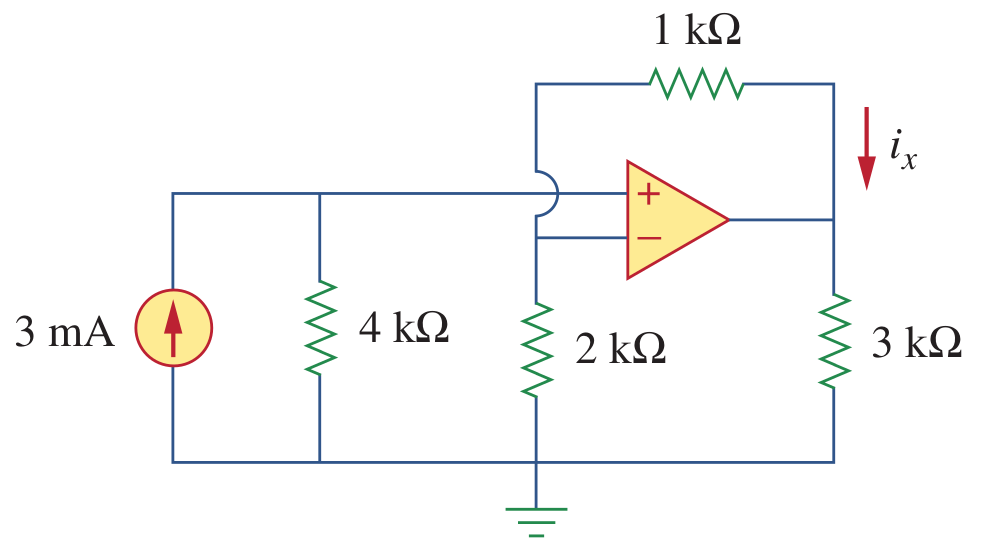
\includegraphics[height=3.6cm]{figure12.png}	
		\end{center}	
		\scalebox{0.8}{Answer: $i_{x}= -6mA \ and \ p_{3k}=108mW$}
		\end{column}
	\end{columns}
\end{tabular}
\end{frame}
% ----------------- NOVA SECÇÂO Section 5.8 Cascaded Op Amp Circuits-----------------------------
\section{Section 5.8 Cascaded Op Amp Circuits}
% ----------------- NOVO SLIDE --------------------------------
\begin{frame}[fragile]
	\frametitle{Cascaded Op Amp Circuits}
\begin{tabular}{ll}
	\begin{columns}
		\begin{column}{1\textwidth}  %%<--- here
		\textbf{Problem 5.63} - Determine the gain \scalebox{1.2}{$\sfrac{v_{o}}{v_{i}}$} of the circuit in Figure below.\\
		\begin{center}
    			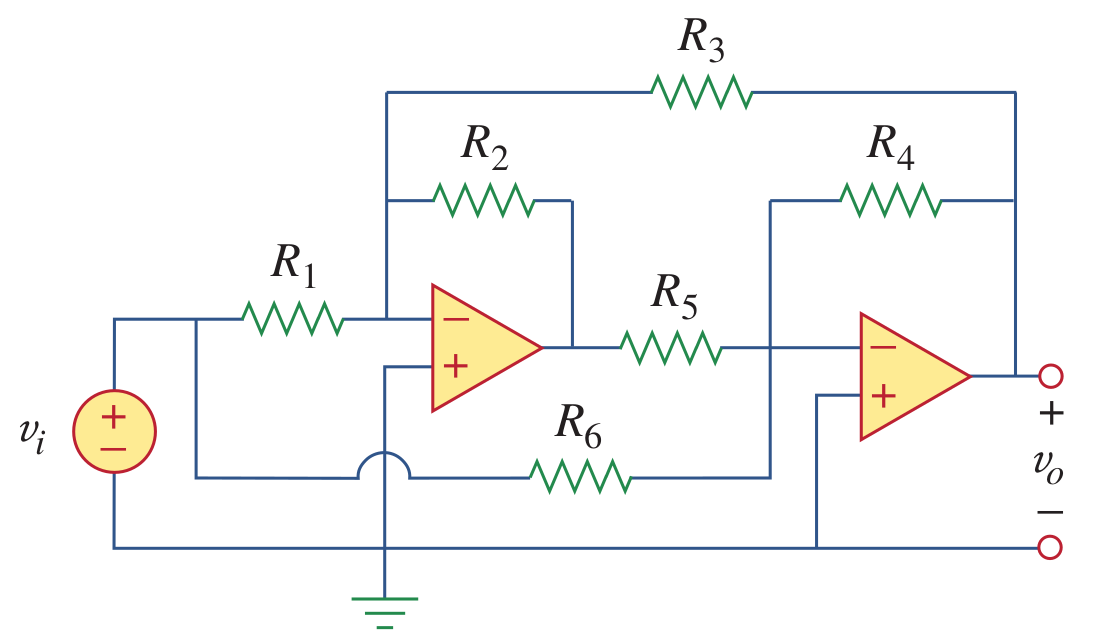
\includegraphics[height=3.6cm]{figure13.png}	
		\end{center}	
		\scalebox{0.8}{Answer: $\frac{v_{o}}{v_{i}}=\frac{\frac{R_{2}R_{4}}{R_{1}R_{5}}-\frac{R_{4}}{R_{6}}}{1-\frac{R_{2}R_{4}}{R_{3}R_{5}}}$}
		\end{column}
	\end{columns}
\end{tabular}
\end{frame}
\end{document} 






